\chapter*{Ejercicio 11}
\addcontentsline{toc}{chapter}{Ejercicio 11}

\section{Parte A}
A partir de la siguiente figura se obtiene la ecuación en diferencias que caracteriza al sistema:

\begin{figure}[H]
    \centering
    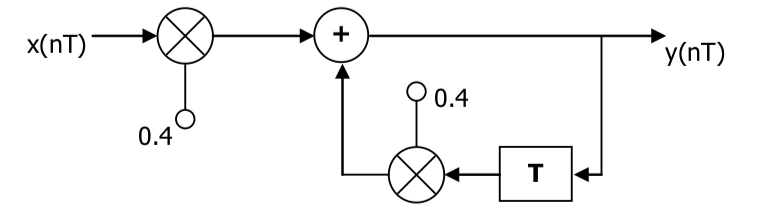
\includegraphics[width=\linewidth]{Ej11.png}
    \caption{Circuito Ejercicio 11}
    \label{fig:e11filtro}
\end{figure}

\begin{equation}
    y(nT) = 0,4x(nT) + 0,4y(nT - T)
\end{equation}

En primer lugar podemos obtener la respuesta impulsiva del sistema reemplazando la entrada con la función delta. Iterando de la siguiente manera y considerando el sistema como relajado:


\begin{align*}
    h(n) = 0,4\delta(n) + 0,4h(n -1)\\
    h(0) = 0,4\delta(0) + 0,4h(-1) = 0,4\\
    h(1) = 0,4\delta(1)+ 0,4h(0) = 0,4^2\\
    h(2) = 0,4\delta(2) + 0,4h(1) = 0,4^3\\
    .\\
    .\\
    .\\
    \boxed{h(n) = 0,4^{n + 1}}\\
\end{align*}

Ahora, considerando una entrada senoidal como la siguiente:

\[
    sen(n\omega T) = 
            \begin{cases}
              sen(n\omega T), & n \geq 0 \\
              0 & n = 0
              
            \end{cases}
\]

se pide obtener una expresión para la ganancia del sistema en régimen permanente. 
Puede escribirse la entrada senoidal de la siguiente manera:

\begin{equation}
    sen(n\omega T) = \frac{1}{2j}(e^{jn\omega T} - e^{-jn\omega T})
\end{equation}{}

Buscando la respuesta a la entrada senoidal:

\begin{equation}
    y(n) = R[x(n)] = R[\frac{1}{2j}(e^{jn\omega T} - e^{-jn\omega T})] \\
    = \frac{1}{2j}R[e^{jn\omega T}] - \frac{1}{2j}R[e^{-jn\omega T}]
\end{equation}{}

Simplificando la notación:

\begin{equation}
    y(n) = \frac{1}{2j}y_{1}(n) + \frac{1}{2j}y_2(n)
\end{equation}{}

donde $y_2(n, \omega) = y_1(n , -\omega) $.

Ahora buscamos $y_1(n)$ convolucionando $x_1(n)$ con $h(n)$:

\begin{equation}
    y_1(n) = x_1(n)\circledast h(n) = \sum_{k=0}^{n} e^{j(n - k)\omega T}0,4^{k + 1} = e^{jn\omega T}0,4\sum_{k=0}^{n} e^{-jn\omega T}0,4^k
\end{equation}{}

La sumatoria anterior es una serie geométrica de los n + 1 primeros términos y puede escribirse de la siguiente forma:

\begin{equation}
y_1(n) = 0,4e^{jn\omega T}[\frac{0,4^{n + 1} * e^{-jn\omega T} * e^{-j\omega T} - 1}{0,4e^{-j\omega T} - 1}] = \frac{0,4^{n + 2} * e^{-jn\omega T} - 0,4e^{jn\omega T}}{0,4e^{-j\omega T} - 1}    
\end{equation}

Si hacemos n tender a infinito se ve que $0,4^{n + 2}$ tinde a 0 por ende queda la siguiente expresión:

\begin{equation}
\Tilde{y_1}(n) = \frac{-0,4*e^{jn\omega T}}{0,4*e^{-jn\omega} - 1}
\end{equation}{}

Luego escribimos $\Tilde{y_1}(n)$ separándola en módulo y fase:

\begin{equation}
\Tilde{y_1}(n) = [|H_1|e^{j\theta _1}] *e^{-jn\omega T}
\end{equation}

Entonces defino:

\begin{equation}
H_1(\omega) = \frac{0,4}{1 - 0,4*e^{-j\omega T}} = \frac{1}{2,5 - e^{-j\omega T}}
\end{equation}

Si se separa el denominador en parte real e imaginaria usando la identidad de Euler y se toma el módulo se llega a la siguiente expresión:
\begin{equation}
    |H_1(\omega)| = \frac{1}{\sqrt{\frac{29}{4} - 5\cos{\omega T}}}
\end{equation}

En tanto que para la fase se llega a lo siguiente:

\begin{equation}
    |\phi(\omega)| = \arctan{\frac{\sin{\omega T}}{\cos{\omega T} - 2,5}}
\end{equation}{}

Mediante python se graficó ambas funciones, el script utilizado se adjunta al final del documento:

\begin{figure}[H]
  \centering
  \begin{minipage}[b]{0.4\textwidth}
    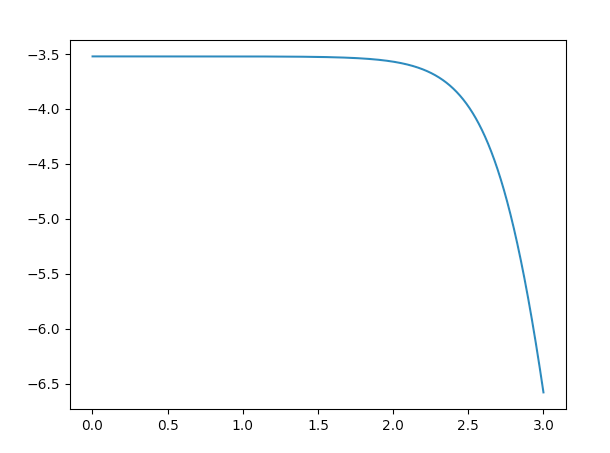
\includegraphics[width=\textwidth]{Ej11_Mag.png}
    \caption{Gráfico Magnitud}
  \end{minipage}
  \hfill
  \begin{minipage}[b]{0.4\textwidth}
    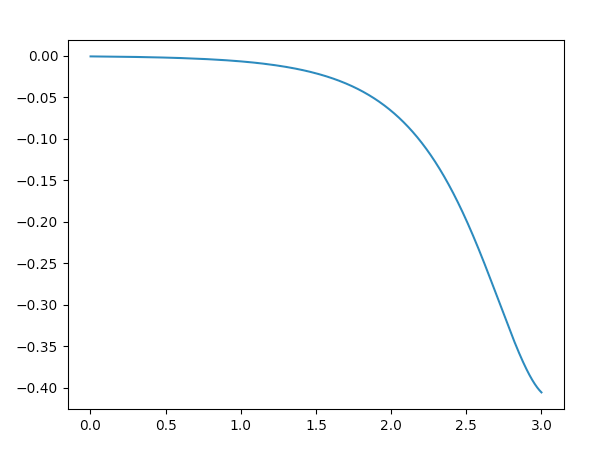
\includegraphics[width=\textwidth]{Ej11_Phase.png}
    \caption{Gráfico Fase}
  \end{minipage}
\end{figure}

\section{Parte B}

Para obtener la frecuencia a la que la ganancia es 3 dB menor a la ganancia en frecuencia 0, primero se obtiene dicha ganancia y luego se despeja de la ecuacion de magnitud: 

\begin{equation}
    H_0 = -3,52dB
\end{equation}{}

\begin{equation}
    \omega = \frac{1}{T} * \arccos{\frac{\frac{29}{4} - \frac{1}{10^{\frac{H_0 - 3}{10}}}}{5}} = 977 Hz
\end{equation}{}

\section{Anexo}

\begin{figure}[H]
    \centering
    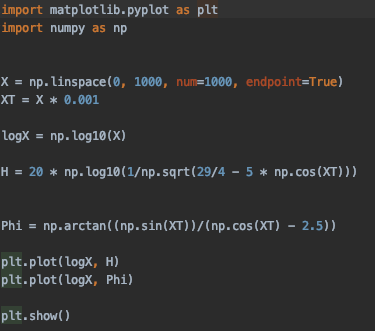
\includegraphics[scale = 0.7]{Codigo.png}
    \caption{Código de gráficos pedidos.}
    \label{fig:my_label}
\end{figure}{}
